% ----------------------------------------------------------
\chapter{Proposta}\label{cap:proposta}
% ----------------------------------------------------------

Este capítulo descreve a arquitetura modular de computação em névoa desenvolvida ao longo deste trabalho. O conteúdo está organizado para apresentar, inicialmente, a visão geral e o papel de cada tipo de nó. Em seguida, são detalhados os componentes, a organização interna dos nós de névoa, os mecanismos de comunicação entre domínios e o fluxo de dados previsto no sistema.

% ----------------------------------------------------------
\section{Visão Geral}
% ----------------------------------------------------------

A arquitetura proposta é composta por três tipos de nós, cada um com responsabilidades distintas no fluxo de dados e na coordenação do processamento distribuído. O nó primário atua como ponto de entrada de um domínio de névoa, gerenciando dispositivos, distribuindo carga e coordenando a comunicação com outros domínios. Os nós de névoa executam o processamento local e oferecem serviços configuráveis para tratamento dos dados. O nó agregador consolida e organiza as informações processadas antes do envio à nuvem.

A Figura~\ref{fig:arquitetura_proposta} apresenta uma visão de alto nível, mostrando o caminho percorrido pelos dados desde os dispositivos na borda até a nuvem, incluindo as interações e responsabilidades de cada tipo de nó.

\begin{figure}[htb]
    \caption{\label{fig:arquitetura_proposta}Visão geral da arquitetura proposta.}
    \begin{center}
        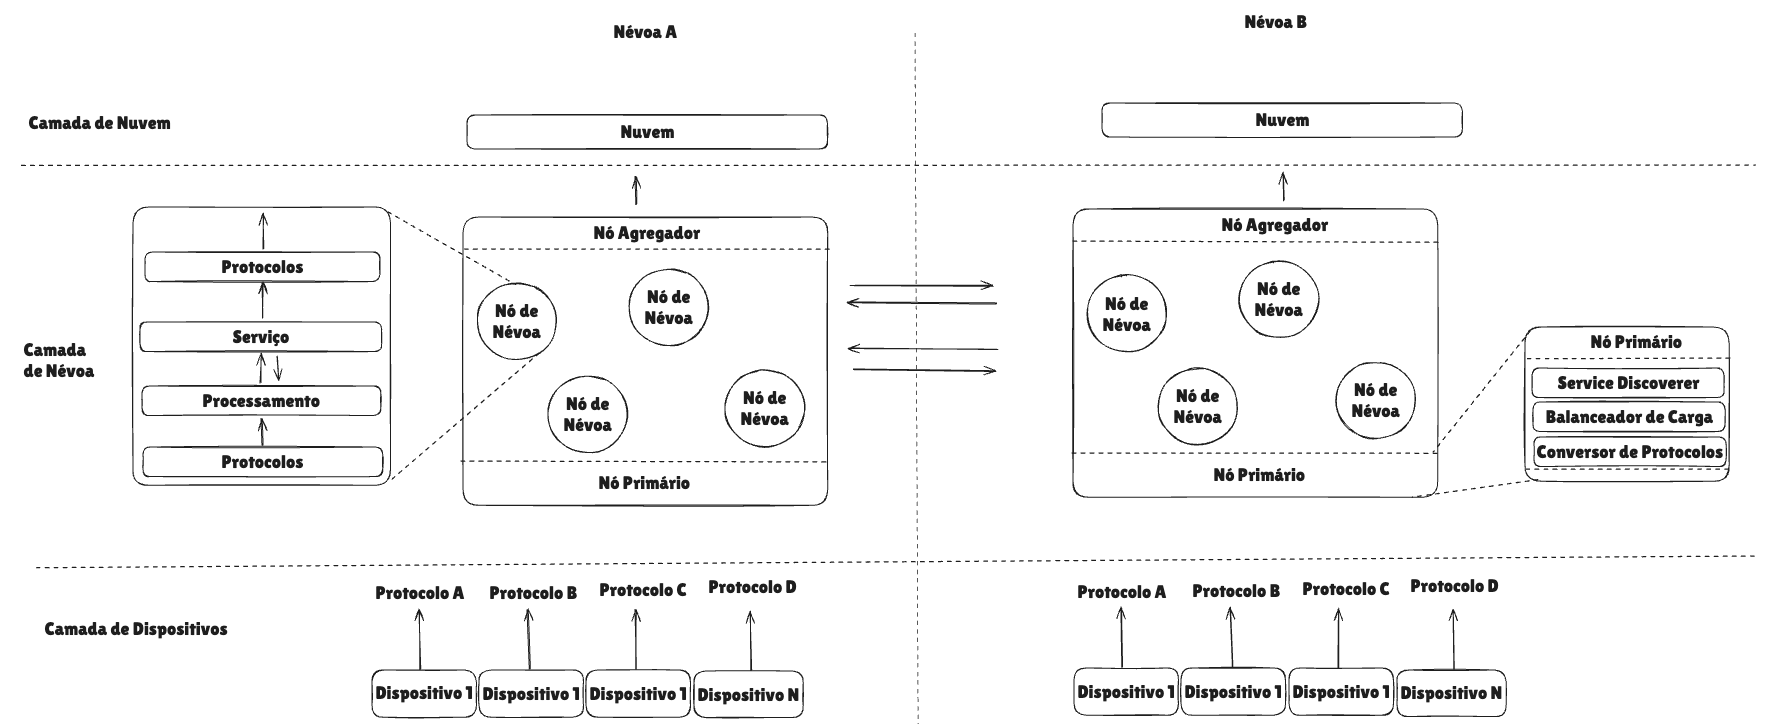
\includegraphics[width=1\linewidth]{images/arquitetura_proposta.png}
    \end{center}
    \fonte{Do autor.}
\end{figure}

% ----------------------------------------------------------
\section{Componentes}
% ----------------------------------------------------------

Esta seção apresenta, em detalhe, as funções e responsabilidades de cada tipo de nó que compõe a arquitetura: nó primário, nós de névoa e nó agregador.

% ----------------------------------------------------------
\subsection{Nó Primário}
% ----------------------------------------------------------

O nó primário funciona como o ponto inicial de contato para dispositivos e novos nós que ingressam em uma névoa. Assim que um nó de névoa é iniciado, ele envia ao nó primário um conjunto de atributos que descrevem sua capacidade, especializações e estado atual de operação. Essas informações são registradas e mantidas para permitir a localização de recursos disponíveis na própria névoa.

Ao receber uma requisição, o nó primário identifica os atributos necessários para o processamento e verifica, entre os nós registrados, quais correspondem ao perfil solicitado. O balanceamento entre os nós locais segue um padrão que procura alternar os destinos de forma equilibrada, em comportamento semelhante a um esquema round robin, sempre respeitando as características solicitadas por cada carga.

Se a análise indicar que não haverá nós suficientes na névoa local para atender à demanda, o nó primário envia uma solicitação para que todos os nós primários de outras névoas informem o estado atual de seus recursos. Esse processo lembra o funcionamento de um protocolo de fofoca, mas é otimizado para reduzir o tráfego de rede, mantendo apenas as trocas essenciais. Com base nas respostas, é selecionada uma névoa remota com disponibilidade, e a requisição é encaminhada para processamento.

O nó primário também é capaz de lidar com diferentes tipos de protocolos, incluindo aqueles que exigem atuação como intermediário na comunicação. Em todos os casos, realiza a adequação inicial do canal recebido, interpretando o conteúdo e convertendo-o para um formato interno uniforme antes de encaminhar para um nó local ou remoto.

% ----------------------------------------------------------
\subsection{Nós de Névoa}
% ----------------------------------------------------------

Os nós de névoa realizam o processamento distribuído e foram organizados em uma estrutura interna baseada em camadas, de forma a facilitar a manutenção e permitir a adição de novas funções sem comprometer o restante do sistema.

A primeira camada, denominada protocolos, é responsável por receber as requisições provenientes do nó primário, realizar as verificações e validações necessárias e repassar as informações para a camada seguinte. Essa estrutura é ilustrada na Figura~\ref{fig:camada_protocolos}, onde diferentes servidores de protocolos alimentam um protocolo padrão utilizado internamente.

\begin{figure}[htb]
    \caption{\label{fig:camada_protocolos}Camada de protocolos de um nó de névoa.}
    \begin{center}
        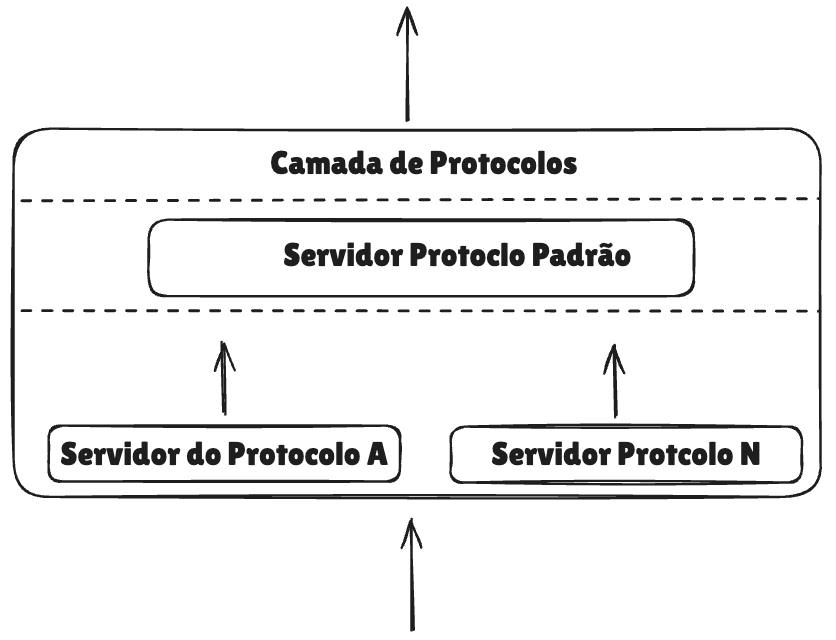
\includegraphics[width=0.7\linewidth]{images/camada_protocolos.png}
    \end{center}
    \fonte{Do autor.}
\end{figure}

A camada de processamento atua como núcleo de coordenação interna, gerenciando a comunicação entre as demais camadas e executando as necessidades específicas do nó de névoa. Essa camada também mantém um mecanismo para consultas internas de dados, permitindo que a camada de serviços acesse apenas as informações estritamente necessárias para seu funcionamento. Além disso, é por meio da camada de processamento que o nó de névoa realiza interações administrativas, como o registro inicial no nó primário. A Figura~\ref{fig:camada_processamento} mostra os principais componentes dessa camada.

\begin{figure}[htb]
    \caption{\label{fig:camada_processamento}Camada de processamento de um nó de névoa.}
    \begin{center}
        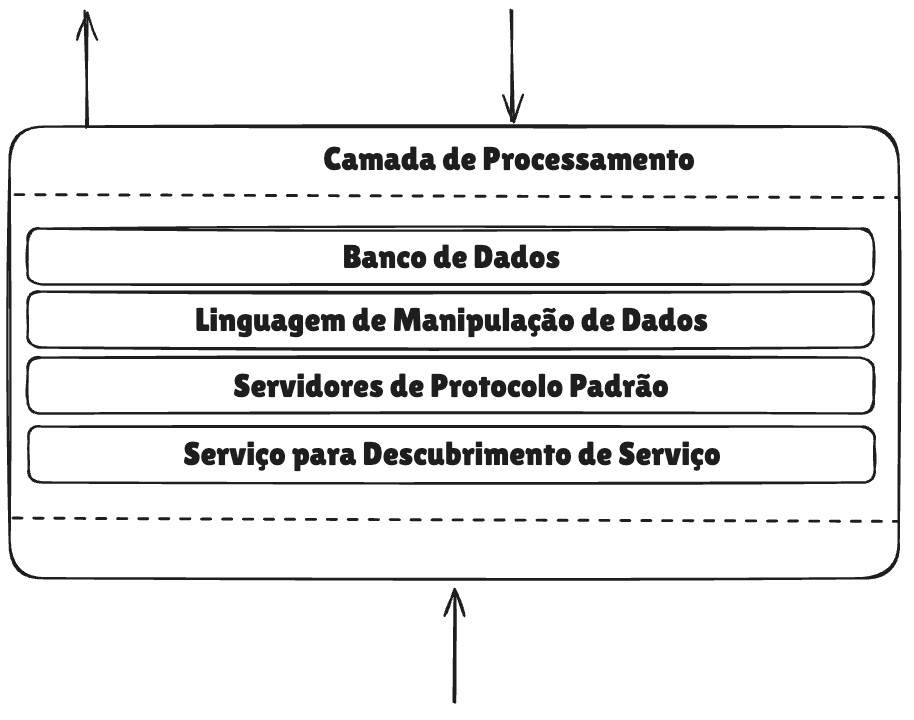
\includegraphics[width=0.7\linewidth]{images/camada_processamento.png}
    \end{center}
    \fonte{Do autor.}
\end{figure}

Na camada de serviços é executada a aplicação que implementa a lógica de pré-processamento dos dados. Utilizando a linguagem de consulta disponibilizada pela camada de processamento, essa camada obtém os dados necessários, executa o tratamento definido pela aplicação e devolve o resultado à camada de processamento, que, por sua vez, ajusta a saída para envio pela camada de protocolos.

% ----------------------------------------------------------
\subsection{Nó Agregador}
% ----------------------------------------------------------

O nó agregador atua como ponto central para receber os resultados pré-processados provenientes dos nós de névoa. Em vez de cada nó de névoa transmitir seus dados diretamente à nuvem, o agregador coleta e organiza essas informações, reunindo-as em um único conjunto consolidado.

Esse processo tem como efeito a redução da quantidade de requisições enviadas à nuvem, agrupando múltiplos envios menores em transmissões mais amplas e organizadas. Embora a redução de tráfego seja um dos resultados esperados, o principal papel do agregador é melhorar o fluxo de comunicação entre a camada de névoa e a nuvem, facilitando o controle, a rastreabilidade e a padronização dos dados enviados.

O nó agregador também pode executar transformações adicionais sobre os dados recebidos, como ajustes de formato, enriquecimento de metadados ou aplicação de funções específicas definidas pela aplicação. Após esse tratamento, os dados são preparados em lotes ou fluxos contínuos e encaminhados à nuvem de acordo com a política de envio configurada.
